% ScholarLens - IEEE conference report skeleton.
% Upload this folder (main.tex, references.bib, and the PNGs from docs/diagrams
% and results/) to Overleaf: New Project -> Upload Project. Overleaf has IEEEtran.
%
% IMPORTANT (from the course guidance): write DETAILED PARAGRAPHS, not bullet
% lists, and write it yourselves (the report must be unplagiarized). The %
% comments under each heading say what to cover; delete them when done.
\documentclass[conference]{IEEEtran}
\usepackage{graphicx}
\usepackage{booktabs}
\usepackage{amsmath}
\usepackage{url}
\usepackage{cite}
\graphicspath{{figures/}}

\begin{document}

\title{ScholarLens: A Multi-Task NLP Assistant for Summarizing, Tagging and Questioning Research Papers}

\author{
\IEEEauthorblockN{Member 1, Member 2, Member 3, Member 4}
\IEEEauthorblockA{Course name, Department, University\\
\{email1, email2, email3, email4\}@university.edu}
}

\maketitle

\begin{abstract}
% 150-200 words, written LAST: problem, what you built (3 tasks, 2 models each),
% data, the headline numbers from results/RESULTS.md, and the main finding.
\end{abstract}

\begin{IEEEkeywords}
summarization, question answering, named entity recognition, transformers, scientific documents
\end{IEEEkeywords}

\section{Introduction}
% 3-4 paragraphs. The real-world problem: the volume of papers, the time to read
% one, why a single tool for summary + key entities + Q&A helps students and
% researchers. Why this is hard (long documents, technical vocabulary, questions
% the paper does not answer). What ScholarLens does in one paragraph, and a
% final paragraph listing your contributions in prose.

\section{Objectives}
% Turn each objective into a measurable statement in a paragraph, e.g. build a
% pipeline that integrates three NLP tasks; fine-tune and compare two transformer
% variants per task; beat simple baselines on at least three metrics per task;
% measure how well a QA model trained on Wikipedia transfers to papers; deliver a
% working demo. Mention the course requirements these satisfy.

\section{Related Work}
% Optional in the guidance but expected in an IEEE paper. One paragraph each:
% long-document summarization \cite{cohan2018discourse,lewis2020bart,raffel2020t5};
% extractive QA and unanswerable questions \cite{rajpurkar2018squad2,liu2019roberta,sanh2019distilbert};
% scientific NER \cite{luan2018scierc,beltagy2019scibert}; dense retrieval \cite{reimers2019sbert,wang2020minilm}.

\section{Approaches and Methods}
\subsection{Preprocessing}
% Describe src/preprocessing.py: LaTeX/citation/URL/figure-reference removal,
% abbreviation-aware sentence splitting, passage construction with overlap, the
% summary quality filter. Explain WHY each step matters. Show a before/after
% example from notebook 00.
\subsection{Abstractive Summarization}
% Encoder-decoder fine-tuning, input truncation to 1,024 tokens and its effect,
% T5 task prefix, beam search settings. Baselines: Lead-3 and TextRank \cite{mihalcea2004textrank}.
\subsection{Scientific Named Entity Recognition}
% Token classification with BIO tags, conversion of SciERC spans, first-sub-word
% labelling, why SciBERT's in-domain vocabulary might help. Baseline: dictionary.
\subsection{Retrieval-Augmented Question Answering}
% Span prediction with a no-answer option, sliding windows (stride), the
% threshold tuned on a held-out split, retrieval of top-3 passages with
% MiniLM vs TF-IDF. Baselines: always-no-answer and TF-IDF sentence.

\section{Workflow}
% Describe Fig.~\ref{fig:arch} and Fig.~\ref{fig:workflow} in paragraphs: the
% data flow at inference time, then how training, model selection and testing
% were separated. Mention tools: GitHub, VS Code, Colab T4, Hugging Face
% Transformers \cite{wolf2020transformers}, Gradio.
\begin{figure*}[t]
\centering
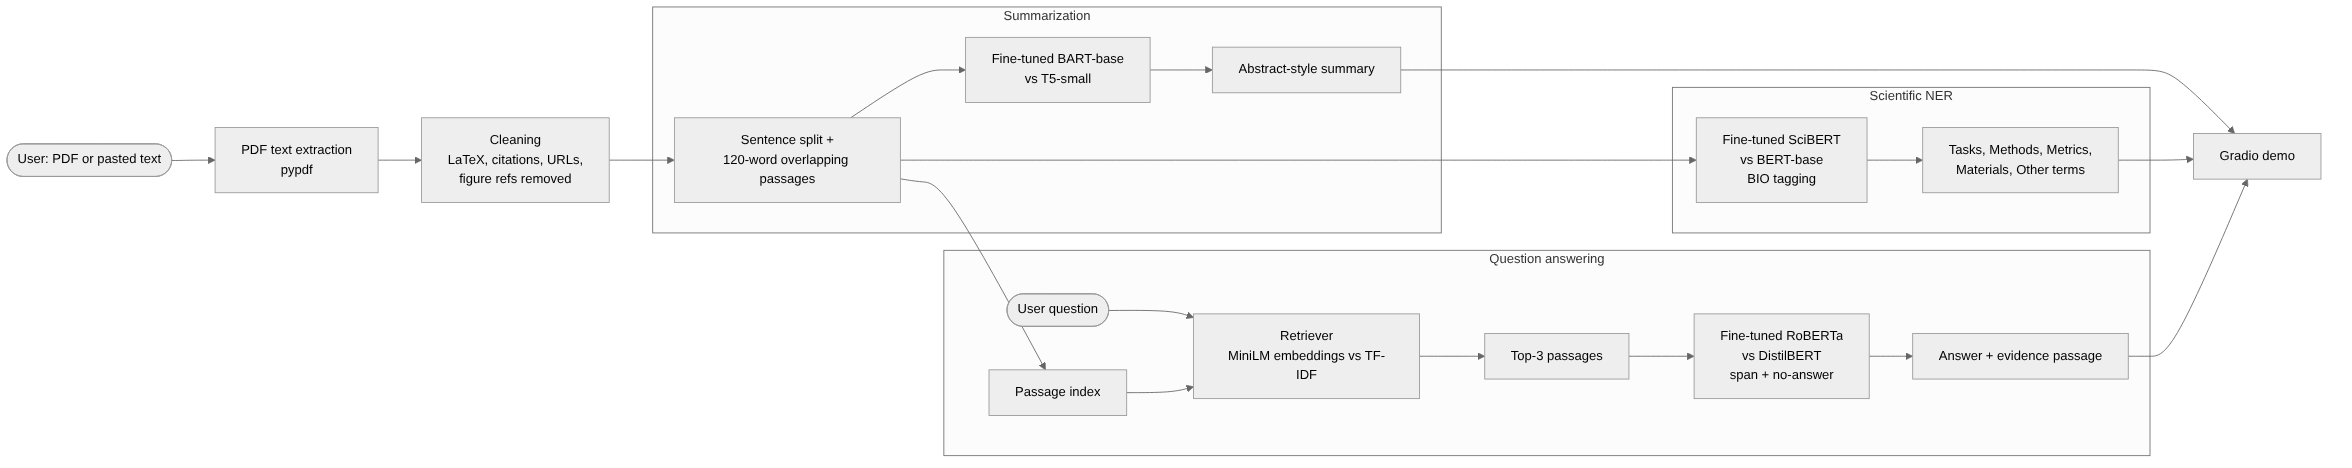
\includegraphics[width=\textwidth]{architecture.png}
\caption{ScholarLens system architecture.}
\label{fig:arch}
\end{figure*}
\begin{figure}[t]
\centering
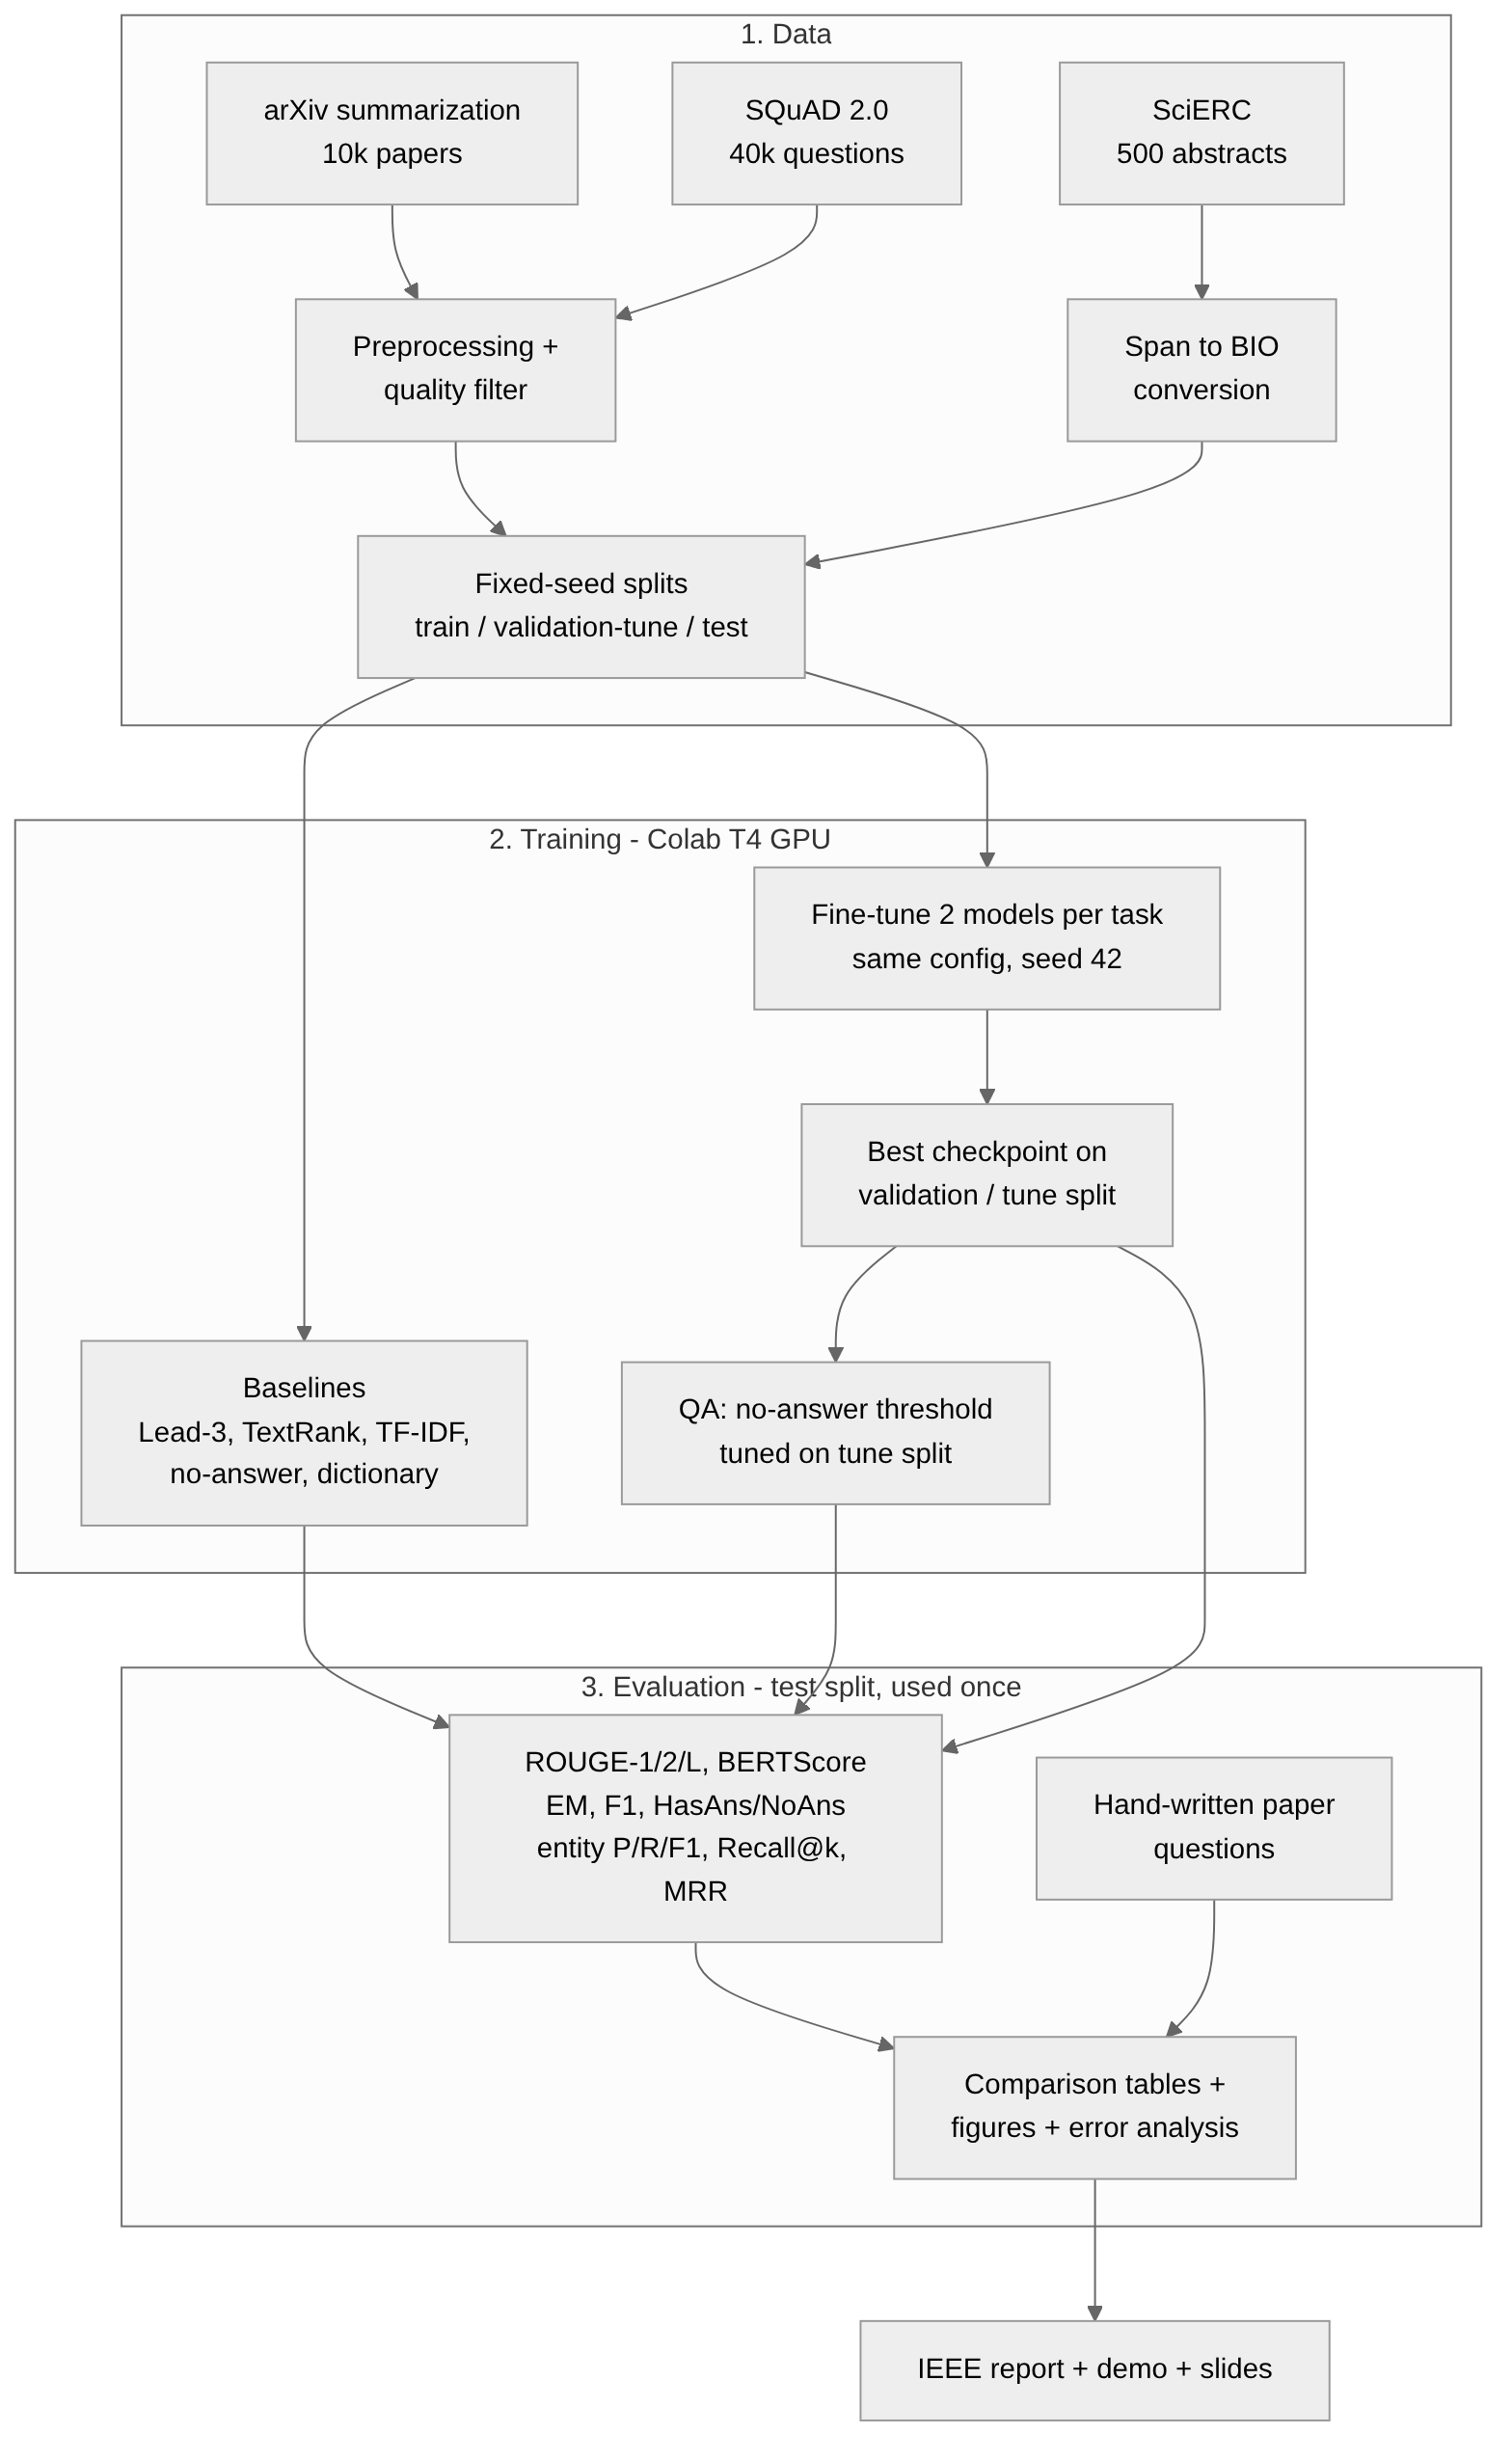
\includegraphics[width=\columnwidth]{workflow.png}
\caption{Training and evaluation workflow.}
\label{fig:workflow}
\end{figure}

\section{Datasets}
% One paragraph per dataset: source and citation \cite{cohan2018discourse,rajpurkar2018squad2,luan2018scierc},
% size you used, splits, cleaning applied, statistics table from
% results/dataset_stats.md, and the sentence count showing >= 50,000 sentences.
% Include the EDA figures (fig_eda_*.png).
\begin{table}[t]
\caption{Dataset statistics (fill from results/dataset_stats.md)}
\centering
\begin{tabular}{lrrr}
\toprule
Dataset & Train & Val/Tune & Test \\
\midrule
arXiv (papers) & & & \\
SQuAD 2.0 (questions) & & & \\
SciERC (sentences) & & & \\
\bottomrule
\end{tabular}
\end{table}

\section{Parameters}
% Table of hyperparameters per model from configs/config.yaml (learning rate,
% batch size, epochs, max lengths, stride, beams, seed) plus GPU and training
% minutes from results/*.json. Explain in a paragraph why you chose them (e.g.
% higher learning rate for T5, more epochs for the small SciERC set).

\section{Evaluation and Discussion}
% Metrics definitions in one paragraph (ROUGE \cite{lin2004rouge}, BERTScore
% \cite{zhang2020bertscore}, EM/F1, entity-level P/R/F1 \cite{nakayama2018seqeval},
% Recall@k, MRR). Then one subsection per task with its table from
% results/comparison_<task>.md, its figure, and DISCUSSION: which model won and
% why, cost vs quality (training minutes), and error analysis with concrete
% examples from results/*_samples.jsonl. Finish with the paper-QA domain-shift
% results and an honest limitations paragraph.
\subsection{Summarization}
\subsection{Question Answering and Retrieval}
\subsection{Named Entity Recognition}
\subsection{Transfer to Real Papers}
\subsection{Limitations}

\section{Conclusion}
% Summarize findings with the key numbers, what you learned, and future work
% (long-document models such as LED, more domain QA data, relation extraction).

\bibliographystyle{IEEEtran}
\bibliography{references}

\end{document}
